%!TEX root = ../main.tex

\section{A primer on the Fake News problem}

Users today when visiting a news outlet or a social network website are commonly confronted with the question as to whether what they are reading is true or false. In this paper, we seek to assist users in tackling this problem by providing a tool to help them spot fake news.

\subsection{News landscape analysis}

Newspapers, magazines and prestigious news outlets have been a reliable news source for centuries. Readers trusted a selected few and the news outlets had an incentive to continue producing good quality information with the risk of loosing their readers to competition. 

Times changed and today.. \note{TODO: present solid references on how the number of news outlets grew, how more fake news are generated and how people trust less and less what they read}

\subsection{Methods used classify Fake News}

\mypara{Content refereeing.} To try to address this problem, some content providers have decided to employ news filtering algorithms for identifying fake news and blocking then from their users. Facebook, Twitter. Facebook has just advertised a system to classify the news based on trustworthiness~\cite{fbrank}. Facebook will begin testing the effort next week by prioritizing news reports in its news feed from publications that users have rated in Facebook surveys as trustworthy. The most ``broadly trusted'' publications—those trusted and recognized by a large cross-section of Facebook users—would get a boost in the news feed, while those that users rate low on trust would be penalized. However, we incur the risks of censorship. Recently, Twitter has been accused of blocking content from right wing circles, and from religious groups. Similar accusation has been made in 2016 to Google, Facebook, and Twitter~\cite{accusedskew}.

\mypara{Fact checkers.} To avoid this, there have appeared services specifically devoted to the identification of fake news and making them available online on some website. Examples of such services include Politifact~\cite{politifact} and FactChecker~\cite{factchecker} focused on US politics, Snopes~\cite{snopes} dedicated to urban myths, and WikiTribune~\cite{wikitribune} to global news. According to a study by the Reuters Institute~\cite{risefackchecking}, in 2016 there were nearly 113 organizations dedicated to fact checking, 90\% of them created since 2010. A fake news organization has even been formed just for this effect, and campaigns for educating users to help them spot fake news. However, the way these systems are build is decoupled from the websites they see, which makes it harder to spot fake news as they visit their preferred news providers. Furthermore, it is sometimes hard for end-users to assess how trustworthy such sources are, making it difficult for users to determine the provenance of the information and reliability of the fact checker. It is sometimes the case that the sources of information are narrowed to specific domains. Another type of system is the Wikipedia, which has already moderation, but relies on a centralized silo of information, with no way for end-users to be able to validate the original provenance of the information.

\mypara{Automatic detection.} There are also emerging automated systems for classifying. But the problem is how to really assess if the results correspond to the truth? It may end up being something where democracy counts. On the other hand it may be possible to build a system where the source of data is already trustworthy and what the system does is to check it. However this is not going to work for real world news where facts have to be validated against external sources before they can be deemed trustworthy. Some previous studies aimed to detect deceptive text on crowdsourced datasets using various techniques, such as stylometric~\cite{stylometric}, semi-supervised learning~\cite{semisupervised}, and linguistic approaches~\cite{linguistic}. Liar~\cite{liar}.

%Centralized solution for someone who stores everything and validates that information for you. Problem of facebook, twitter being accused of bias.

\subsection{A novel approach: Distributed Verifiable Claims}

\note{TODO: João, colocar imagens em papers não funciona como em blog posts. Tu colocas a imagem e tens de fazer referência no texto. Se fores ver a versão render do paper vais ver que a imagem não paarece aqui.}

\begin{figure}[t]
  \centering
  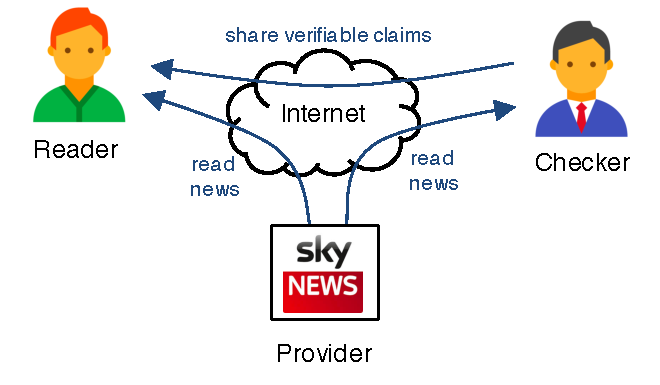
\includegraphics[width=0.9\columnwidth]{figures/model.pdf}
  \vspace{-10pt}
  \caption{Fake news detection based on verifiable claims.}
% \vspace{-0.3cm}
  \label{fig:model}
\end{figure}

Verifiable Claims are a proposal by W3C. 

\note{TODO:
  - Explicar o que são as Verifiable Claims e fazer ref ao RFC
  - Explicar os shortcommings (json-ld schemas === não funciona offline)
  - Explicar que continua a exigir uma autoridade para guardar as claims
  - Introduzir então as Distributed Verifiable Claims que usam "bleeding edge" e novel approach das Blockchains e P2P para permitir que funcione tudo distribuido
}

\subsection{Objectives and Requirements}

In order to build a system for fake news detection based on verifiable claims, several challenges need to be overcome:

\mypara{Censorship resistance:} How to prevent someone from blocking access to the content or preventing issuers from submitting their reviews to the system.

\mypara{Security:} How to ensure that the news are not altered, that the content is not modified, and that it is possible for users to be sure that a certain given content has been endorsed by someone they really trust.

\mypara{Resilience:} We need to ensure that our system survives attacks from powerful organizations and is able to preserve the content persistently for a long time span.

\mypara{Source anonymity:} How to provide anonymity protection? Talk about privacy. 

\mypara{Incentives} Talk about incentives that must be aligned. Talk about sustainability.
